% The short-comings of other solutions are somewhat a continuation of the problem description

% * things from the knowledge-base: redux, flux, angular, meteor, linked-data
%    * instead of in problem-description (more abstract there)
\chapter{State of the Art}

\section{Frameworks and Architecture}

\subsection{Model-View-Controller}\label{ref:mvc}

You probably already are familiar with the classical model-view-controller architecture, but for the sake of completeness a short overview will be given here. The pattern mainly consists of three types of building blocks (as can also be seen in figure \ref{fig:mvc}): \todo{TODO sources}

\begin{description}
  \item[controllers] contain the lion's share of the business logic. User input gets handled by them and they get to query the model. Depending on these two information sources they decide what messages to send to the the model, i.e. the controller telling the model to change. Usually there's one controller per view and vice-versa.
  \item[models] hold the application's state and make sure it's consistent. If something in the data changes, it notifies views and controllers depending on it. These notifications can be parametrized, telling the dependants what changed.
  \item[views] are what the outside world/user's get to see. When the model changes, the view get's notified and -- depending on the data passed along and what it reads from the model --  updates accordingly.
  Especially in html-applications, views (and thereby controllers) tend to be nested (e.g. the entire screen -- a column -- a widget in it -- a button in the widget)
\end{description}

Note that there's a wide range of different instances/interpretations of the architectural patterns can organise models/views/controllers differently. Further down, in section \ref{ref:angular-mvc} you can find one of these (angular's MVC) described in more detail.

\begin{figure*}
\centering
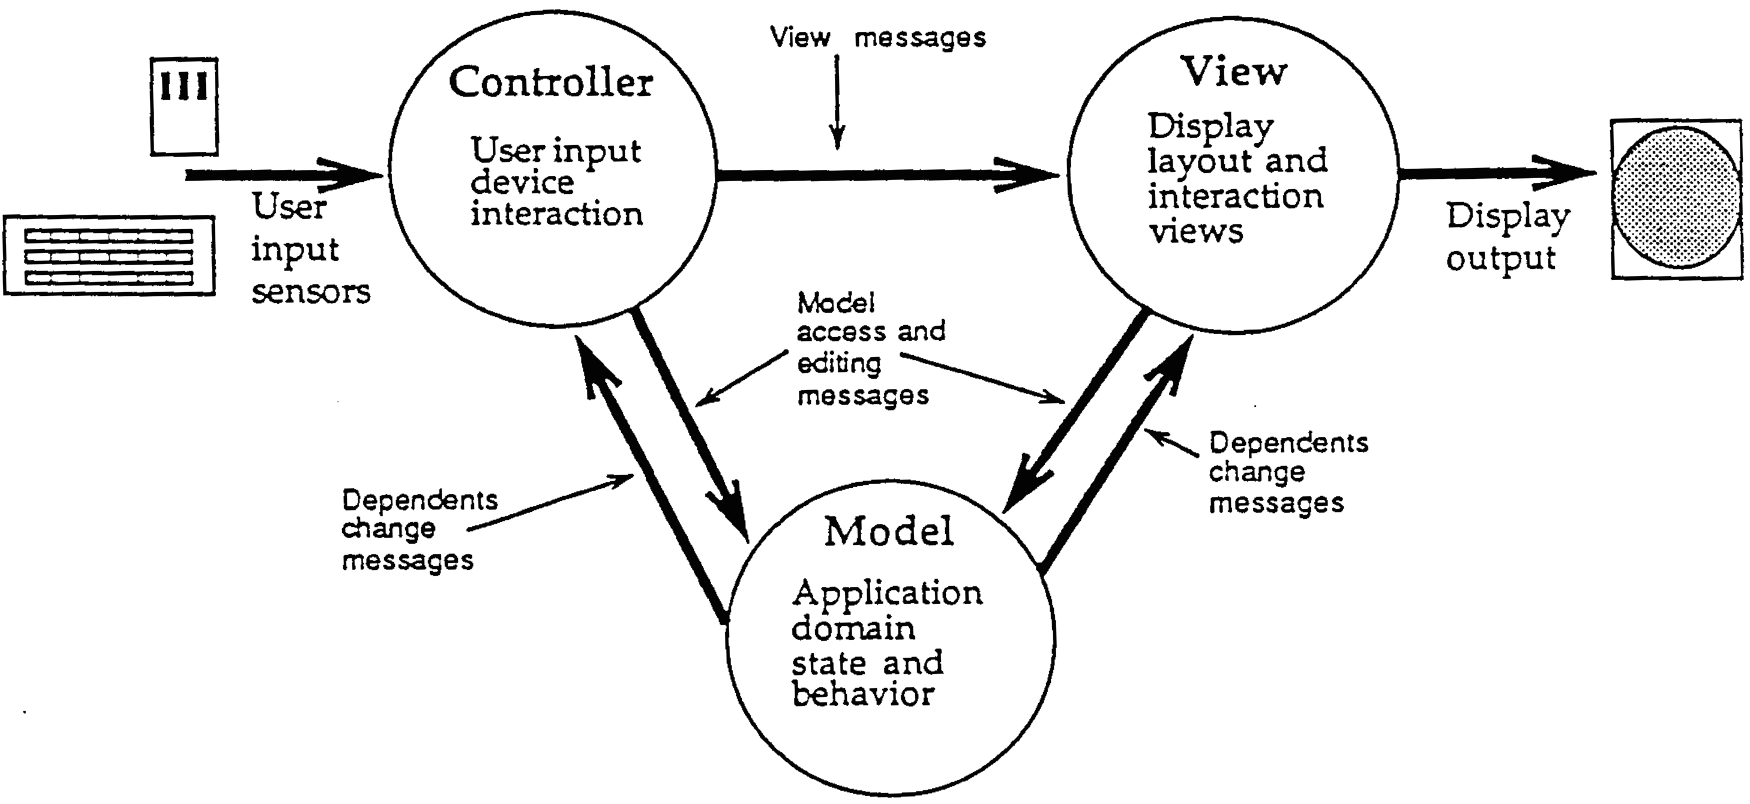
\includegraphics[width=1.0\textwidth]{figures/mvc.png}
\caption[MVC-architecture]{MVC-architecture (Krasner and Pope, 1988)}
\label{fig:mvc}
\end{figure*}
\todo{ TODO krasner and pope 1988: http://heaveneverywhere.com/stp/PostScript/mvc.pdf }

\subsection{Model-View-ViewModel}\label{ref:mvvm}

This architectural pattern, also known as ``Model-View-Binder'', is similar to MVC but puts more emphasis on the seperation between back-end and front-end. It's parts are as follows (and can be seen in fig. \ref{fig:mvvm}):\todo{TODO sources}

\begin{description}
  \item[The model] is the back-end business-logic and state. It can be on a different machine entirely, e.g. a web-server.
  \item[The view-model] contains the front-end logic and state. It is a thin binding layer, that processes inputs and that manages and provides the data required by the view.
  \item[The view] is a stateless rendering of the data retrieved from the view-model; in the case of some frameworks, this happens via declarative statements in the view's templates, that automatically get updated when the data in the view-model changes. User-input events raised in the view get forwarded to the view-model.
\end{description}

\begin{figure*}
\centering
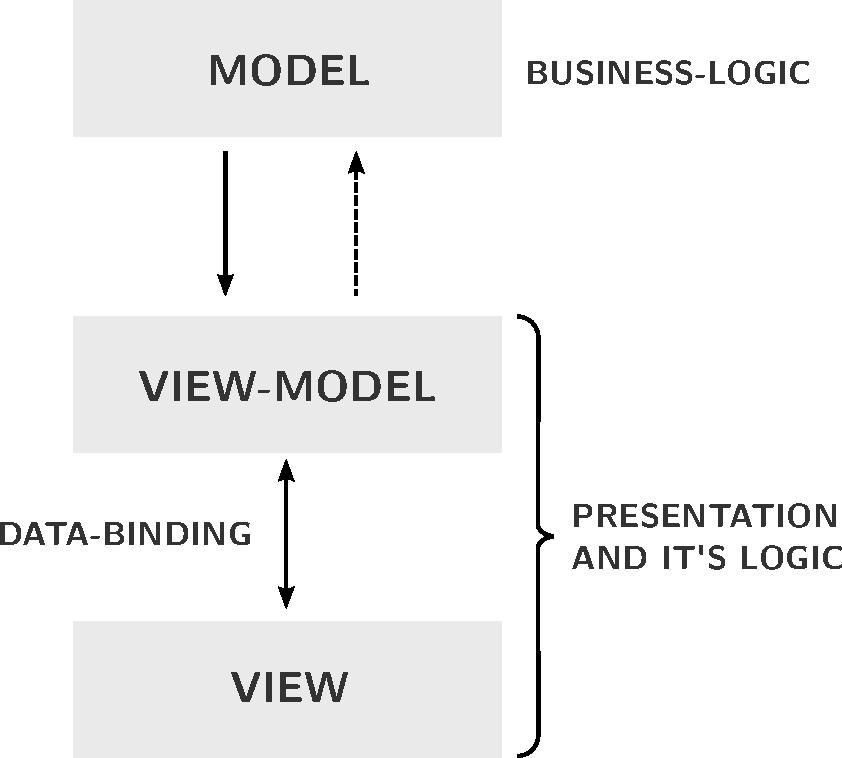
\includegraphics[height=8cm]{figures/mvvm.pdf}
\caption[MVC-architecture]{ MVVM-architecture (diagram \href{https://en.wikipedia.org/wiki/File:MVVMPattern.png}{adapted from wikimedia}\footnotemark{})}
\label{fig:mvvm}}
\end{figure*}
\footnotetext{\url{https://en.wikipedia.org/wiki/File:MVVMPattern.png}}

\subsection{Angular 1.x MVC}\label{ref:angular-mvc}

\todo{Too much detail! Move a lot of these details to later chapters (e.g. "solution » ng best practices" or "solution » why we moved from ng to ng-redux")}

Angular 1.x is a javascript-framework that roughly follows the MVC/MVVM architectures, but has a few conceptual variations and extensions.

On the View-side of things there's templates (see fig. \ref{fig:ng-template} for an example from the webofneeds-codebase). These are either specified in an html-file and then later linked with a controller or are a string in the declaration of something called a "directive" (which are custom html tags or properties). Every template has a scope object bound to it and can contain expressions -- e.g. those in curly braces -- that have access to that scope object. For the example in fig. \ref{fig:ng-template} this means, that -- in the HTML that the user gets to see -- the curly braces will have been replaced by the result of \texttt{self.post.getIn(['won:hasContent','won:hasTextDescription'])} (the \texttt{getIn} is there because \texttt{post} is an \fnurl{https://facebook.github.io/immutable-js/}{immutable-js} object). Practically every time the result of that expression changes, angular will update the displayed value. Basically every expression causes a ``watch'' to be created (this can also be done manually via \texttt{\$scope.watch}). On every ``digest-cycle'' checks all of these watch-expressions for changes and then executes their callbacks, which in the case of the curly-braces causes the DOM-update.

Beyond the curly braces, angular also provides a handful of other template-utilities in the form of directives. For instance the property-directive \texttt{ng-repeat} allows iterating over a collection as follows:

\begin{verbatim}
<div ng-repeat="el in collection">{{el.someVar}}</div>
\end{verbatim} 

Or, similiarly, \texttt{ng-show="someBoolVar"} conditionally displays content.

Note that these template-bindings are bi-directional, i.e. the code in the template can change the the values in the scope. Additionally, templates/directives can be nested within each other. By default, their scopes then use javascript's \fnurl{https://developer.mozilla.org/en/docs/Web/JavaScript/Inheritance_and_the_prototype_chain}{prototypical inheritance} mechanism, i.e. if a value can't be found on the template's/directive's scope, angular will then go on to try to get it from the on the one wrapping it (and so on)
This allows writing small apps or components where all data-flows are represented and all code contained in the template. For medium-sized or large apps however, the combination of bi-directional binding and scope inheritance, can lead to hard-to-follow causality, thus hard-to-track-down bugs and thus poor maintainability. More on that later. % in section X
\todo{TODO add reference to that subsection} 
Also, using scope inheritance reduces reusability, as the respective components won't work in other contexts any more. \todo{move critique of bi-dir binding and inheritance to later chapter}

\todo{ TODO get syntax-highlighting to work in figures (see comment in .tex) } % \begin{lstlisting}[style=json]}
\begin{figure*}
\centering
\begin{verbatim}
...
<h2 class="post-info__heading"
  ng-show="self.post.getIn(['won:hasContent','won:hasTextDescription'])">
    Description
</h2>
<p class="post-info__details"
  ng-show="self.post.getIn(['won:hasContent','won:hasTextDescription'])">
    {{ self.post.getIn(['won:hasContent','won:hasTextDescription']) }}
</p>
...
\end{verbatim}
\caption{Excerpt of angular-template}
\label{fig:ng-template}
\end{figure*}

For all but the very smallest views/components the UI-update logic will be contained in angular's controllers, however. They are connected with their corresponding templates via the routing-configuration (more on that later \todo{ref to routing-subsection}) or by being part of the same directive \todo{ref to directive-subsection}. Controllers have access to their template's scope and vis versa %(see section X
\todo{ref to controllerAs discussion}
%)
Theoretically it's possible to pair up / reuse controllers with different templates, but this can lead to hard-to-track-down and I'd advise against doing that.
When nesting templates and thus they're associated controllers, actually it's the controllers that form the prototypical inheritance chain. Thus, if a variable isn't found on the controller respectively it's scope, the default is to check on it's parent('s), up to the root-scope. Note that scopes can be defined as isolated in the routing config \todo{ref to routing/isolated-scope section} to avoid this behaviour, which I'd recommend for predicatability- and thus maintainability-reasons.

\todo{ can be reused with different template, but that rarely happens and tends to lead to hard-to-track-down bugs.}
\todo{nesting templates (not directives?) -- how does it work anyway?}

\todo{move controllerAs advice to later chapter}
\begin{comment}
Controllers have access to their template's scope via the variable \texttt{scope} that they get in their factory-function/constructor. 
Alternatively, they can be bound e.g. as \texttt{self} to the scope by specifying \texttt{controllerAs: "self"} in the routing-/directive-config. This avoids the situation where you specify a variable on the wrong object and then the template-expression can't find it (e.g. if you miss that \texttt{this} in a bound function points to the controller-object instead of the scope) Generally speaking, using \texttt{controllerAs} makes mistakes/bugs less likely. 
\end{comment}

Now, with models/scopes, views/templates and controllers we would have a classical MVC-framework (see section \ref{ref:mvc}). However, angular also has the concept of services: Essentially, they are objects that controllers can access and that can provide utility functions, manage global application state or make http-requests to a web-server. Controllers can't gain access to each other -- except for nesting / prototypical inheritance -- but they can always request access to any service (via dependency injection; more on
that later\todo{ref to subsection}). Examples of services are \texttt{\$scope} that, amongst others, allows registering custom watch-expressions with angular outside of templates (see fig. \ref{fig:ng-simple-ctrl} for an example). Another example for a service would be our custom \texttt{linkeddata-service.js} that can be used to load and cache RDF-data\footnote{see section \ref{data-on-won-nodes} for more on RDF}.


\todo{ TODO get syntax-highlighting to work in figures (see comment in .tex) } % \begin{lstlisting}[style=javascript]}
\begin{figure*}
\centering
\begin{verbatim}
var myApp = angular.module('myApp', []);
myApp.controller('PostController', function ($scope) {
  $scope.post = { text: 'heio! :)' };
  $scope.$watch('post.text', function(currentText, prevText) {
    console.log('Text has been edited: ', currentText);
  });
});
\end{verbatim}
\caption{Example of a very simple controller and usage of the \texttt{\$scope}-service}
\label{fig:ng-simple-ctrl}
\end{figure*}

With services added to the mix, we can also view the angular framework through the lense of MVVM (see section \ref{ref:mvvm}), with templates as views, scopes and controllers as view-models and services as models or as proxies for models on a web-server (as we did with the \texttt{linkeddata-service.js}).

% \todo{ TODO get syntax-highlighting to work in figures (see comment in .tex) } % \begin{lstlisting}[style=javascript]}
\begin{figure*}
\centering
\begin{verbatim}
myApp.config(['$routeProvider',
  function($routeProvider) {
    $routeProvider.
      when('/landingpage?:focusSignup', {
        templateUrl: 'app/components/\
          landingpage/landingpage.html',
        controller: 'LandingpageController'
      }).
      when('/post/?postUri', {
        templateUrl: 'app/components/\
          post/post.html',
        controller: 'PostController'
      }).
      otherwise({
        redirectTo: '/landingpage'
      });
  }]);
\end{verbatim}
\caption{Example of routing-configuration in Angular 1.X}
\label{fig:ng-simple-routing}
\end{figure*}

% todo move this to later chapters (e.g. a section on module systems)

Note, that Angular 1.x uses it's own module system to manage directives, controllers and services. If you include all modules directly via \texttt{<script>}-tags in your \texttt{index.html}, this mechanism makes sure they're executed in the correct order. However, this also means, that if you want to combine all your scripts into one \texttt{bundle.js}\footnote{
Bundling for instance helps to reduce the number of HTTP-requests on page-load and thus it's performance. It can be done by using a build-tool like browserify, webpack or jspm plus a module system like AMD, CommonJS or the recently standardized ES6-modules (see \url{http://www.ecma-international.org/ecma-262/6.0/#sec-imports})}
}
you'll have to specify the same dependencies twice -- once for your bundling module system and once for angular's, as can be seen in figure \ref{fig:ng-duplicate-dependencies}.\todo{ref number doesn't match figure's}

\begin{figure*}
\centering
\begin{verbatim}
/* es6 imports for bundling */

import angular from 'angular'
import createNeedTitleBarModule from '../create-need-title-bar';
import posttypeSelectModule from '../posttype-select';

//...

class CreateNeedController { /* ... */ }

//...

/* angular module declaration */

export default angular.module(
  /* module's name: */
  'won.owner.components.createNeed', 
  [ /* module's dependencies: */
    createNeedTitleBarModule,
    posttypeSelectModule,
    // ...
  ])
  .controller(
    'CreateNeedController', 
    [
      '$q', '$ngRedux', '$scope', // services for ctrl
      CreateNeedController // controller factory/class
    ])
.name;
\end{verbatim}
\caption{Example of module- and controller-declaration in \texttt{create-need.js}}
\label{fig:ng-duplicate-dependencies}
\end{figure*}


% TODO stopped here


\begin{comment}
in the problem-descripion: list challenges that need to be tackled by web applications:

* seperation of concerns
  * suitability for collaboration
  * reusability of code
* move processing to client / minimal number of requests (justification for js-apps)
* networking
* optimize page load:
  * less http-requests -> bundling
  * smaller size -> minification
  * precompiling templates
* managing dependencies between scripts -> module systems
* simplicity / a low number of concepts / gentle learning curve
* predictability / maintainability


\end{comment}









\todo{TODO reference ng docu}

\begin{comment}

    * [ ] views - templates + controller
	* [ ] controllers / factory methods
        * [x] somewhere between MVVM-viewmodels and MVC-controllers
		* [ ] best practice: avoid putting too much code into these
	* [ ] routing 
        * [ ] how controllers+html-templates are brought together
    * [ ] directives (component style or attributes)
        * [ ] explain with example of modal?
        * [ ] preferable to view+controller as code for both + bundling of them is in one place (~react components)
    * [x] services ~MVVM-model
    * [x] arguably more mvvm than mvc
    * [ ] rather steep learning curve. 
        * [ ] especially to use it well. there's many pitfalls for people just starting out with it to produce a code-base that's hard to maintain later on. (personal experience with smartengine-code and own code)
        * [ ] TEXT?: as concrete usage example angular solves a wide range of different problems (routing, state managment, networking, display,...) and it does so with an equally wide range of mechanisms. Redux on the other hand, has one a very small number of mechanisms, that it uses to solve all these problems similiarly (e.g. routing-information is part of the redux-state)
        * [ ] TEXT: ... As you can see angular is rather complex in it's architecture and contains quite a few pitfalls for the unwary newcomer. As such, it has a rather steep learning curve.
    * [x] bi-directional binding
    * [ ] auto-injection into scope via things like ng-model
    * [x] scoping / hierarchy of controllers
    * [x] scope-inheritance and it's problems!
    * [ ] modules and dependency-injection
      * [ ] "Bringing it all together..."
      * [ ] need to include each and every javascript file (in the right order?). everything is loaded with quite a few http-requests. can be bundled though
        * make sure to use strict mode to allow bundling
      * [ ] no tree-shaking
      * [x] redundant to es6-module system
    * [x] services
      * [x] keep global state
      * [x] wrap access utilities to server-APIs
      * [x] access to utility functions that can be injected (instead of being attached to the window)
    * [ ] controllers
      * [x] both controllers and partly models (is angular actually mvvm?)
      * [x] can be reused with different template, but that rarely happens and tends to lead to hard-to-track-down bugs.
      * [ ] mostly used at view level. below that directives provide more atomic bundling of template and code.
    * [x] templates
    * [ ] filters
      * { probably not necessary to explain }
    * [ ] directives
      * [ ] bundle controller and template in one file
      * [ ] register custom html-tag (unless used in attribute, like ng-show/-class/-..., or class mode)
    * [ ] routing
      * [ ] html-fragments
      * [ ] ui-router (?) (are we using or have we used it?)
\end{comment}

\subsection{Meteor}

\todo{ dunno if necessary? }

\subsection{React}

\begin{comment}
  * atomic components
  * vdom allows not needing to deal with dom-state just with defining one mapping from app-state to desired html. react takes care of calculating a minimal set of updates (by diff'ing the current vdom against the vdom that produced the previous dom-state (?))
\end{comment}

\subsection{Flux}

\begin{comment}
  * quite a learning-curve
  * actions
  * dispatcher
    * there are many different implementations of these (the one by fb, the one by yahoo,...)
  * stores
    * waitFor
    * dependencies between these can be hard to understand
    * lot of overhead
    * side-effect free? if so, do as much as business logic as possible here.
  * views
    * most dispatchers / setups are geared to be used with redux
\end{comment}


\subsection{Redux}\label{ref:redux}

\begin{comment}
  * http://redux.js.org/
  * can be super-simple (give trivial example)
  * easy to learn (it's only one event-bus/dispatcher, one reduction-function)
  * ideally used with immutable data for model (to avoid bugs due to pass-by-reference and later modification)
  * doesn't deal with side-effects by default (see ACs and actors later)
  * (action-creators (for pre-processing))
  * actions
  * dispatcher
  * reduction function
    * synchronous (can't do asynch side-effects here)
    * (supposed to be) side-effect free. do as much as business logic as possible here.
  * components
\end{comment}

\subsection{Ng-Redux}\label{ref:ng-redux}

\begin{comment}
  * https://github.com/wbuchwalter/ng-redux
  * angular 1.X for rendering instead of flux
  * good for migrating
  * duplicate imports if using es6 (though not ng-redux inherent)
  * explain binding into routing, setup of watches, importance of one way bindings
\end{comment}


\subsection{Elm}

\begin{comment}
  * previous (at time of designing)
  * current
\end{comment}

\subsection{CycleJS MVI}

\begin{comment}
* driver's are similiar to actors?
\end{comment}

\todo{ move this to methodology chapter? }

\todo{ http://redux.js.org/ \\
 https://github.com/angular-redux/ng-redux }
